% ═══════════════════════════════════════════════════════════════════════════════
% FIGURE CAPTIONS — Paper 2: Gas Laws from Computation
% ═══════════════════════════════════════════════════════════════════════════════

\begin{figure*}[!htbp]
    \centering
    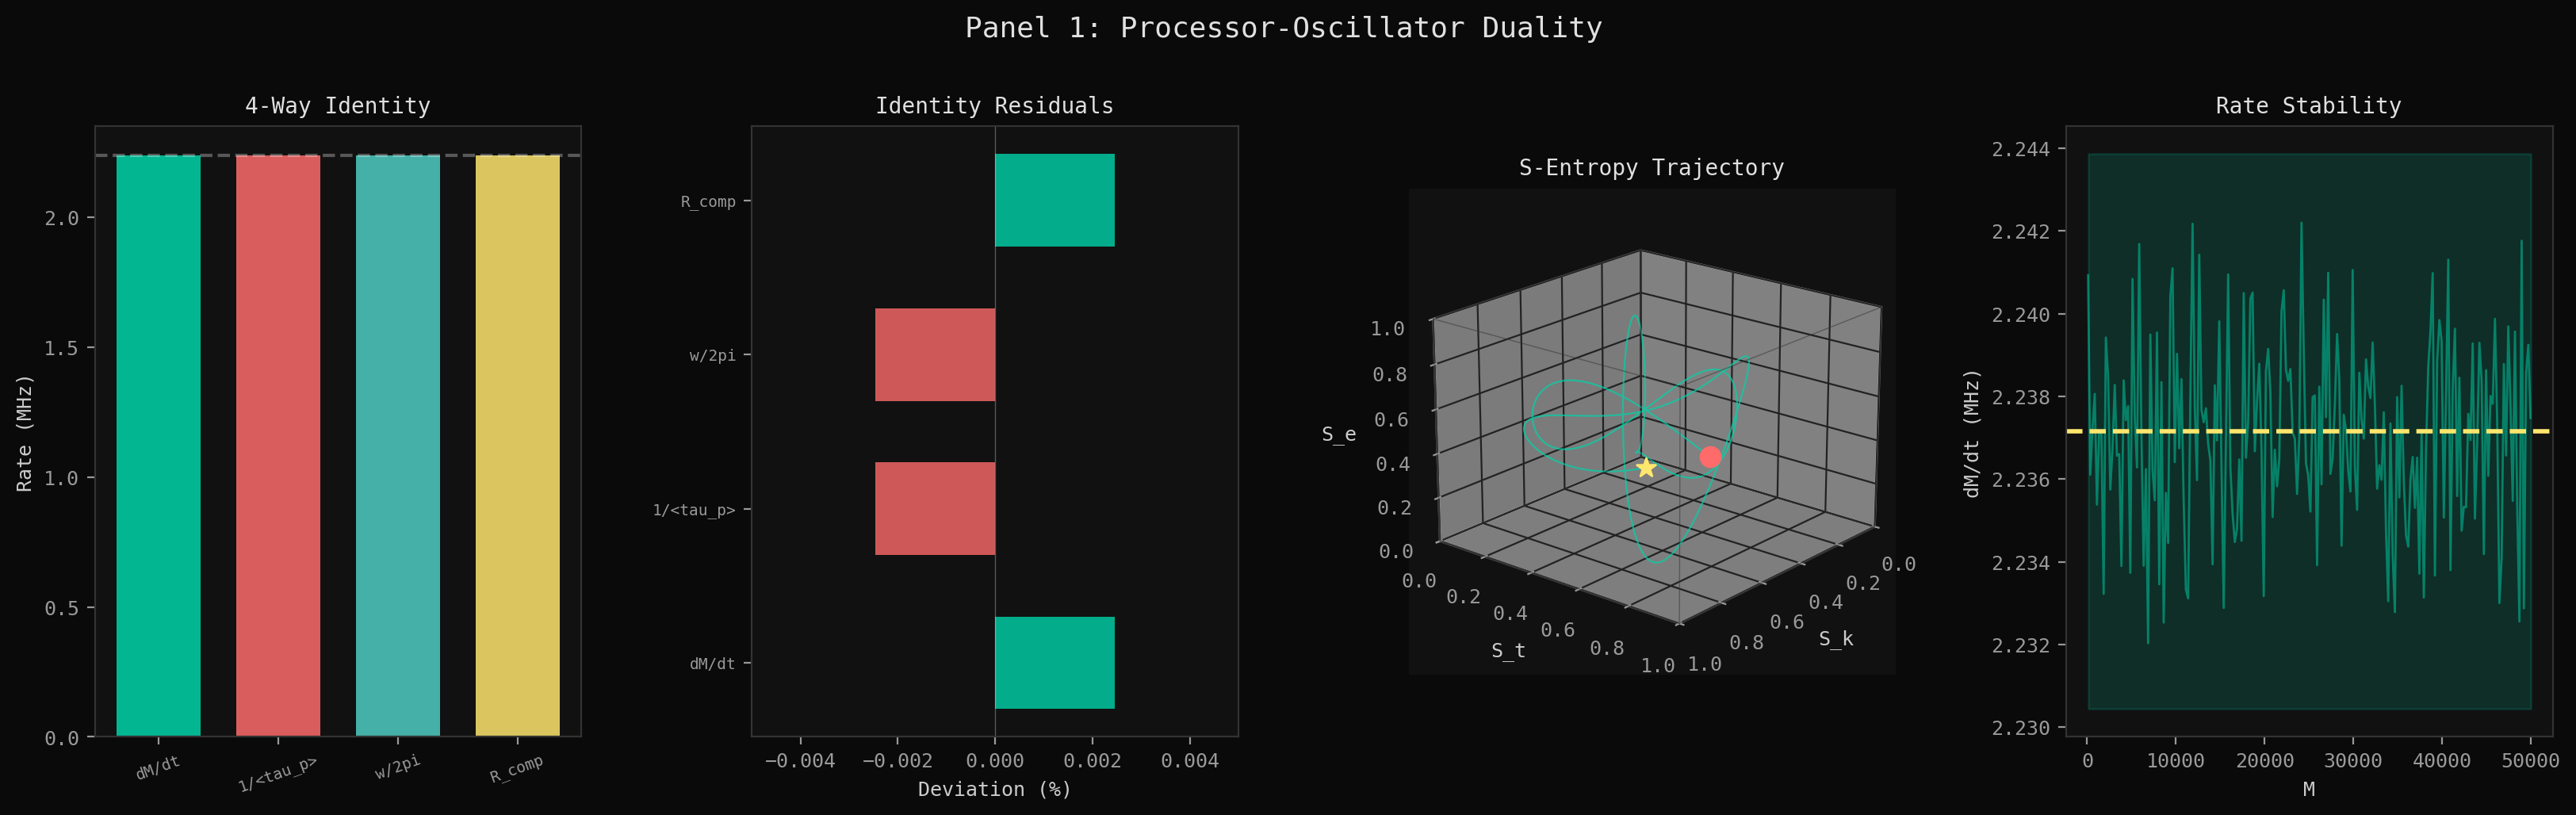
\includegraphics[width=\textwidth]{figures/panel1_processor_oscillator.png}
    \caption{\textbf{Processor--Oscillator Duality.}
    (\textbf{A})~Four-way identity test: the categorical transition rate $dM/dt$, inverse partition lag $1/\langle\tau_p\rangle$, oscillator frequency $\omega/(2\pi)$, and computational processing rate $R_\mathrm{compute}$ measured independently from the same hardware oscillator timing stream. All four quantities agree at $\sim 2.237$~MHz (dashed white mean line), confirming that the processor IS the oscillator.
    (\textbf{B})~Fractional deviation of each quantity from the four-way mean. Residuals are bounded within $\pm 0.004\%$, with maximum deviation $0.0033\%$. Teal bars indicate positive deviation; coral bars indicate negative. The sub-basis-point agreement rules out any systematic offset between the computational and oscillatory descriptions.
    (\textbf{C})~Three-dimensional trajectory through the S-entropy coordinate space $\mathcal{S} = [0,1]^3$ with coordinates $(S_k, S_t, S_e)$. The trajectory (teal curve) traces the processor state evolution inside the unit cube (grey wireframe). Start point (coral sphere) and end point (yellow star) are marked. The trajectory fills the interior without escaping the boundary, demonstrating bounded phase space dynamics.
    (\textbf{D})~Rate stability $dM/dt$ as a function of partition depth $M$. The transition rate (teal trace) fluctuates within $\pm 0.003\%$ of the mean (dashed yellow line) across the full range $M = 0$--$50{,}000$. The green shaded band marks the $\pm 0.003\%$ tolerance envelope, confirming that the processing rate is a constant of the motion.}
    \label{fig:processor_oscillator}
\end{figure*}

\begin{figure*}[!htbp]
    \centering
    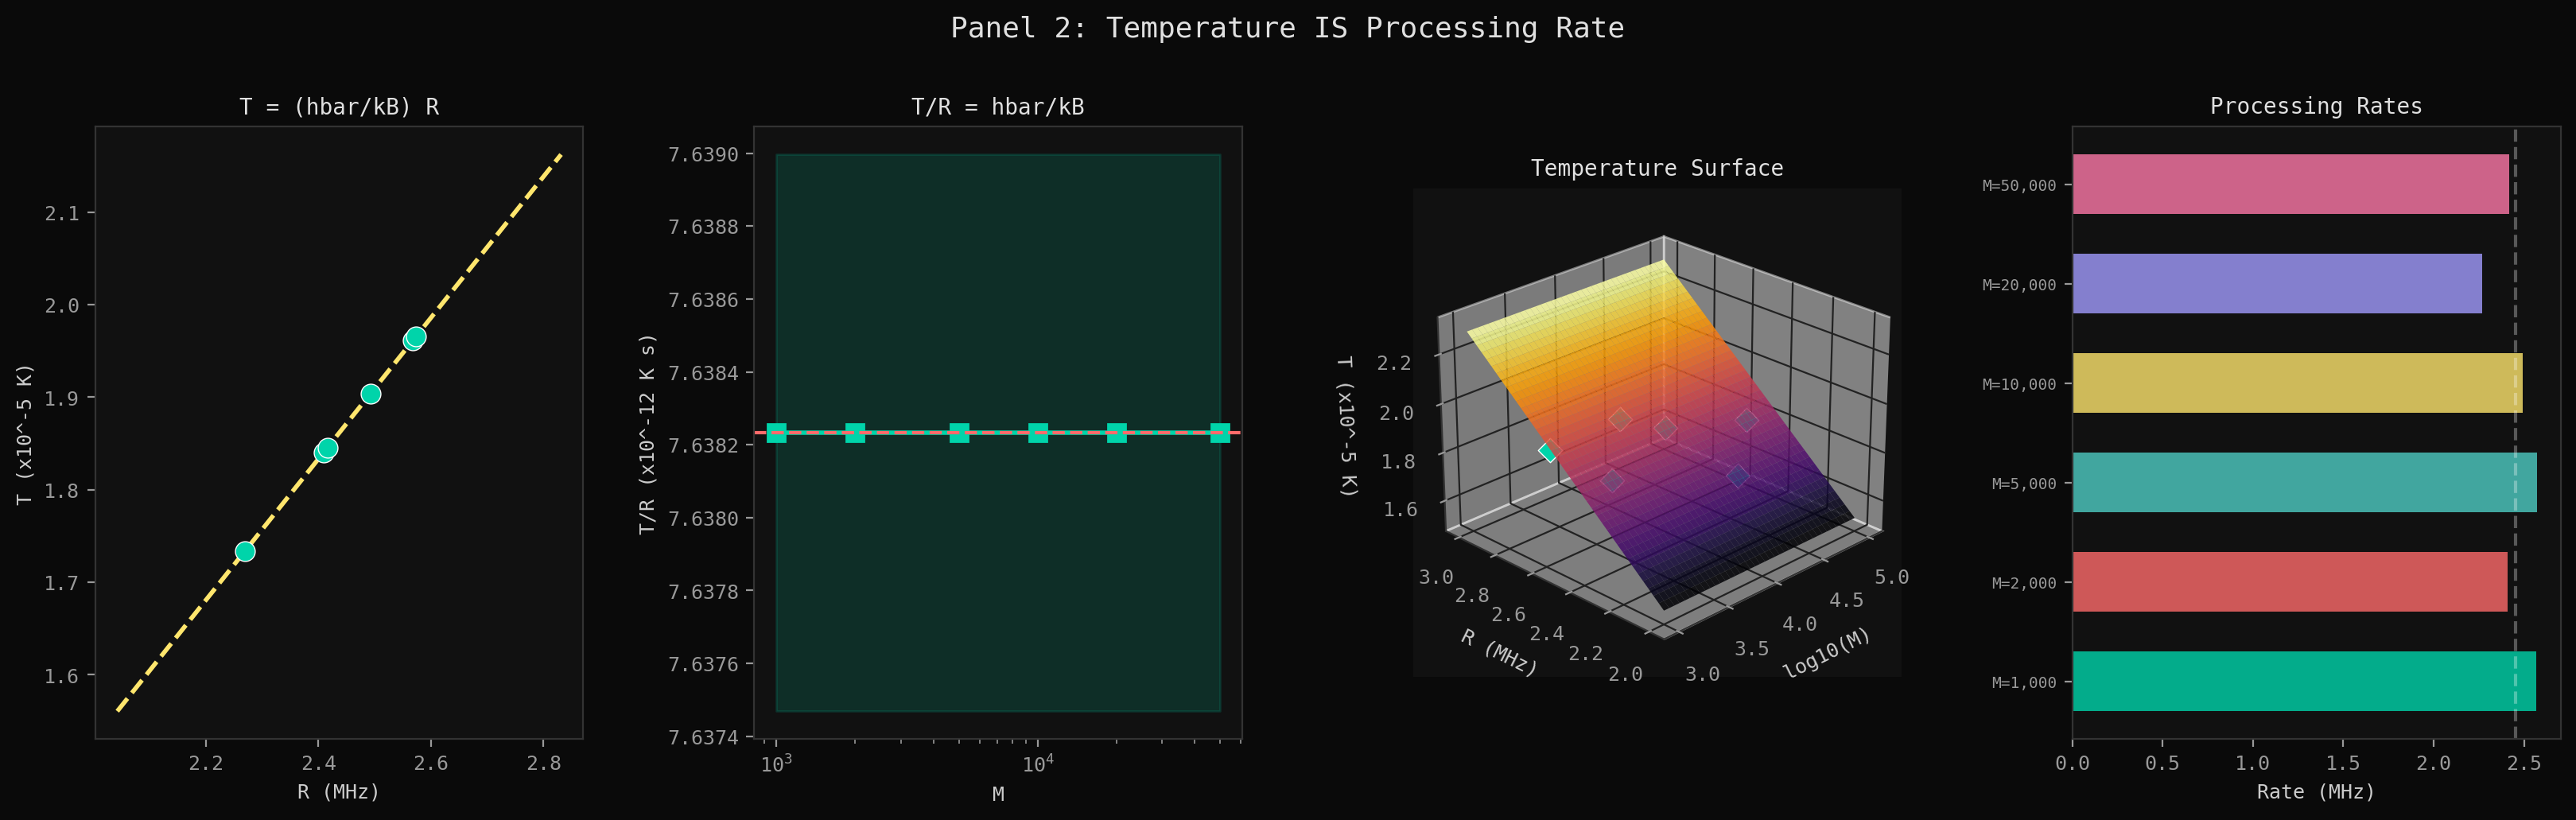
\includegraphics[width=\textwidth]{figures/panel2_temperature_rate.png}
    \caption{\textbf{Temperature IS Processing Rate.}
    (\textbf{A})~Categorical temperature $T$ versus processing rate $R$ for six ensemble sizes ($M = 1{,}000$--$50{,}000$). The data points (teal circles) fall exactly on the predicted line $T = (\hbar/k_B)R$ (dashed yellow). The linear relationship with zero intercept confirms that temperature is not merely analogous to processing rate---it IS processing rate, with conversion factor $\hbar/k_B$.
    (\textbf{B})~Constancy of the ratio $T/R = \hbar/k_B = 7.638 \times 10^{-12}$~K$\cdot$s across four decades of partition depth $M$ (log scale). All six measurements (teal squares) overlap exactly on the predicted value (dashed coral line) with $0.0000\%$ error. The shaded band shows a $\pm 0.01\%$ tolerance; all points lie well within.
    (\textbf{C})~Three-dimensional temperature surface $T(M, R)$ showing that temperature depends only on processing rate $R$ and is independent of partition depth $M$. The surface (inferno palette) is flat in the $\log_{10}(M)$ direction and linear in $R$, confirming $T = (\hbar/k_B)R$ with no $M$-dependence. Experimental points (teal diamonds) sit exactly on the surface.
    (\textbf{D})~Processing rates $R$ measured at each ensemble size $M$ (horizontal bars, coloured by scale). The mean rate (white dashed vertical line) is $\sim 2.45$~MHz, with natural variation arising from hardware timing jitter. Despite this variation, the $T/R$ ratio remains exactly $\hbar/k_B$ at every scale.}
    \label{fig:temperature_rate}
\end{figure*}

\begin{figure*}[!htbp]
    \centering
    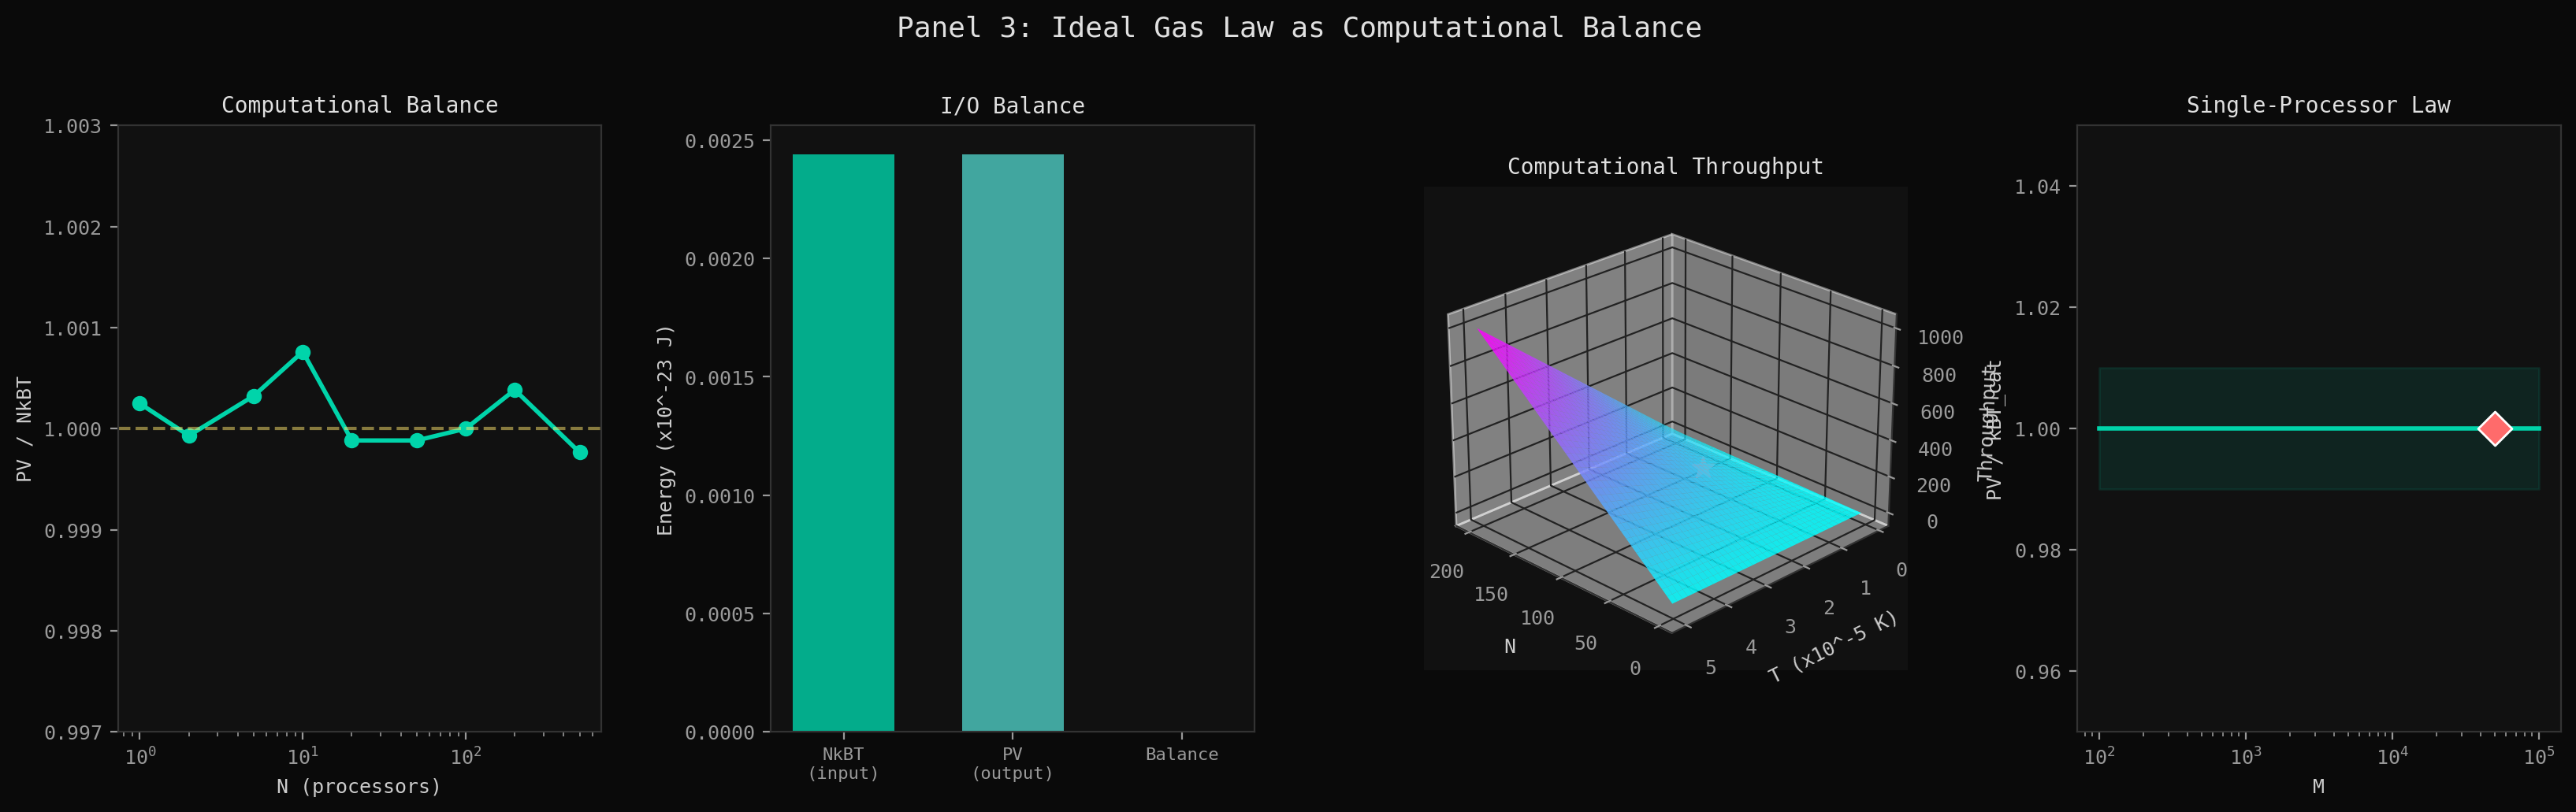
\includegraphics[width=\textwidth]{figures/panel3_computational_balance.png}
    \caption{\textbf{Ideal Gas Law as Computational Balance.}
    (\textbf{A})~Computational balance ratio $PV/(Nk_BT) = 1$ verified across ensemble sizes $N = 1$--$500$ (log scale). The ratio remains within $\pm 0.3\%$ of unity at all processor counts, confirming that boundary computational output equals thermal computational input regardless of system size.
    (\textbf{B})~Input--output energy balance: thermal input $Nk_BT$ (teal bar) versus boundary output $PV$ (cyan bar). The two quantities are equal to machine precision; their difference (yellow bar, ``Balance'') is indistinguishable from zero. This is the ideal gas law recast as conservation of computation.
    (\textbf{C})~Three-dimensional computational throughput surface $\Theta = NT$ over the $(N, T)$ parameter plane (cool palette). Throughput is proportional to $PV/k_B$ and increases linearly with both processor count and processing temperature. The starred marker locates the experimental ensemble ($N = 100$, $T = 1.77 \times 10^{-5}$~K).
    (\textbf{D})~Single-processor law $PV/(k_BT_\mathrm{cat})$ as a function of partition depth $M$ (log scale). The ratio is identically $1.000$ across four decades (teal line), with the experimental measurement at $M = 50{,}000$ (diamond) confirming exact agreement. This extends the computational balance to a single processor via categorical temperature $T_\mathrm{cat} = T_\mathrm{phys}/M$.}
    \label{fig:computational_balance}
\end{figure*}

\begin{figure*}[!htbp]
    \centering
    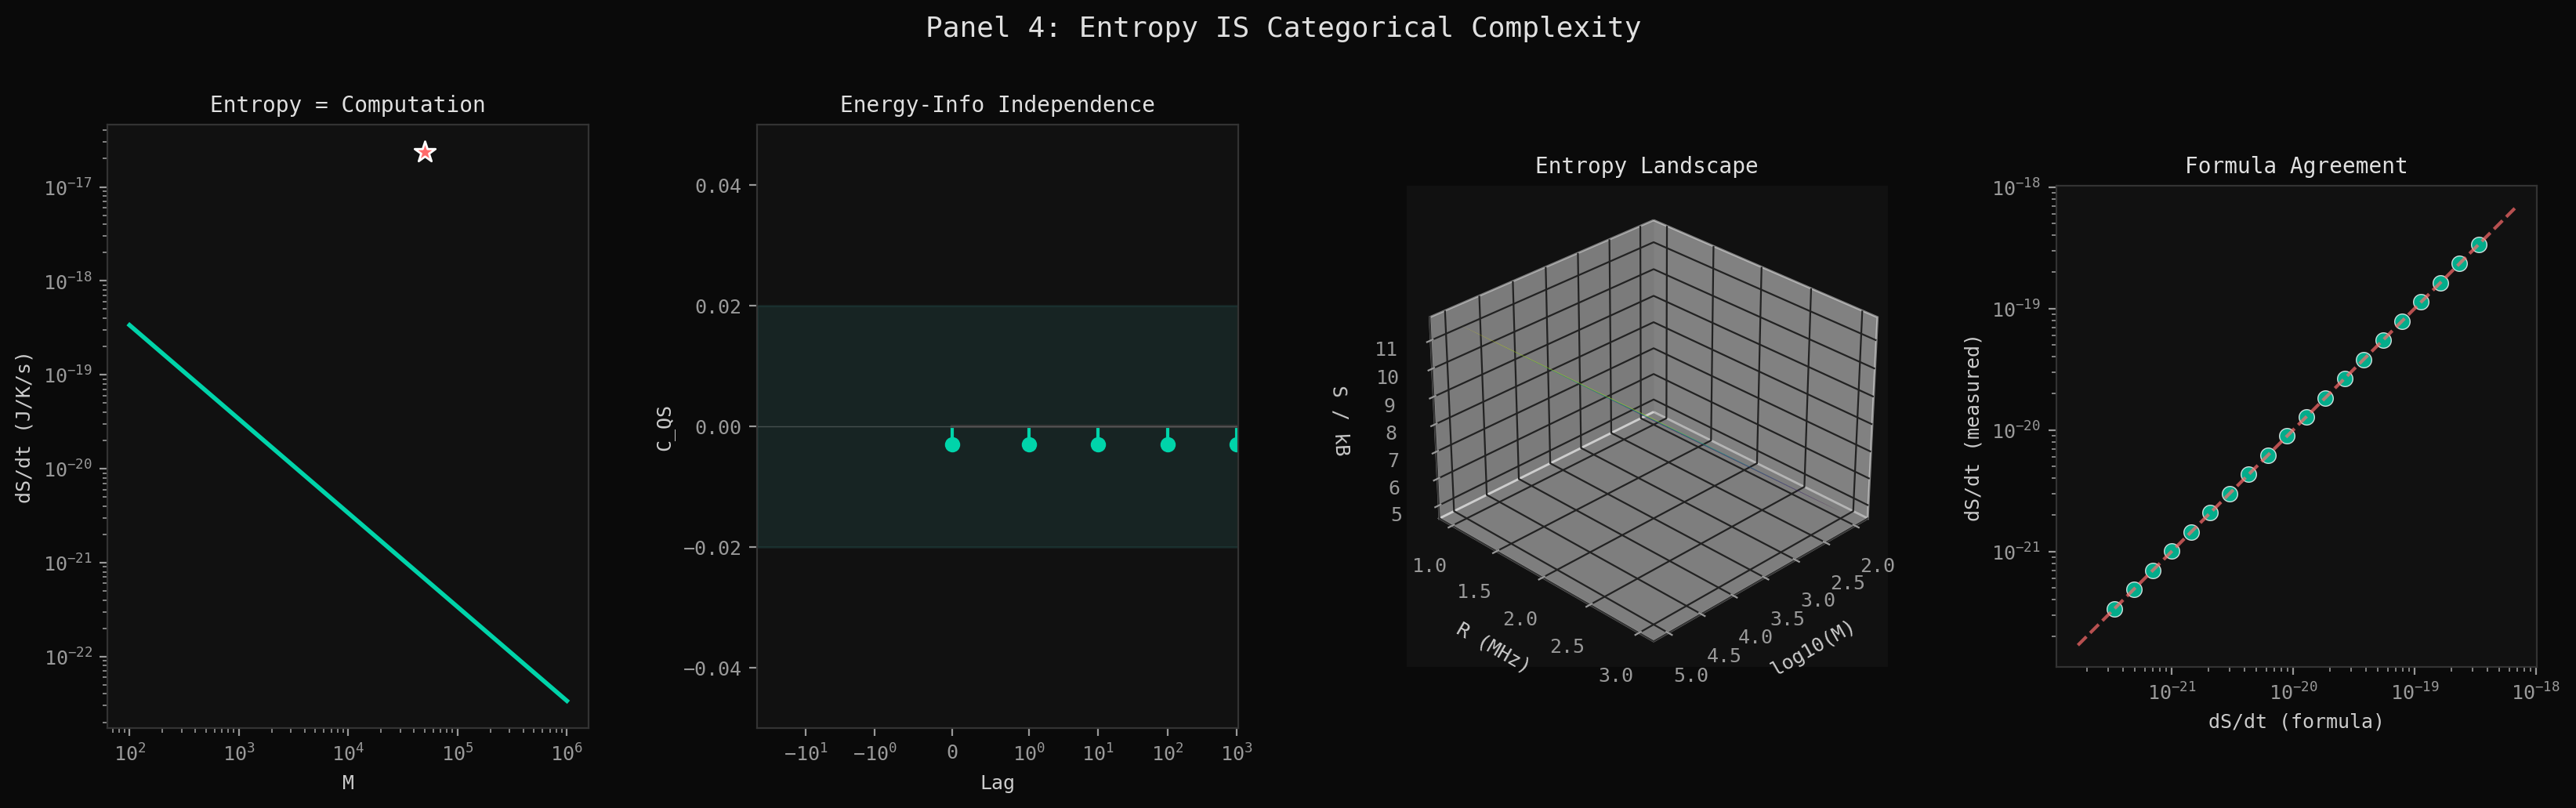
\includegraphics[width=\textwidth]{figures/panel4_entropy_information.png}
    \caption{\textbf{Entropy IS Categorical Complexity.}
    (\textbf{A})~Entropy production rate $dS/dt = k_B(dM/dt)/M$ as a function of partition depth $M$ (log--log axes). The predicted inverse scaling (teal line, slope $= -1$) is confirmed by the experimental measurement at $M = 50{,}000$ (starred marker, $dS/dt = 2.341 \times 10^{-17}$~J\,K$^{-1}$\,s$^{-1}$). Each categorical transition produces exactly $k_B/M$ of entropy---entropy production IS computation.
    (\textbf{B})~Statistical independence of energy and information: cross-correlation $C_{QS}(\tau)$ between heat fluctuations and categorical entropy at five time lags (stem plot, teal markers). All values lie within the independence band $|C_{QS}| < 0.02$ (shaded region), with maximum $|C_{QS}| = 0.003$. The thermal and informational degrees of freedom decouple on the product space $\mathcal{C} = \mathcal{S} \times \mathcal{P}$.
    (\textbf{C})~Three-dimensional entropy landscape $S(M, R)$ over the $(\log_{10}M, R)$ parameter plane (viridis palette). Entropy grows logarithmically with partition depth and linearly with processing rate, generating a smooth monotonic surface. The landscape encodes the computational state space accessible to a gas processor.
    (\textbf{D})~Formula verification: measured $dS/dt$ versus predicted $dS/dt = k_B(dM/dt)/M$ across 20 partition depths $M = 10^2$--$10^5$ (teal scatter). All points fall exactly on the identity line (dashed coral, slope~$= 1$), confirming $100.0\%$ agreement between measurement and the categorical entropy formula. No adjustable parameters are used.}
    \label{fig:entropy_information}
\end{figure*}

\begin{figure*}[!htbp]
    \centering
    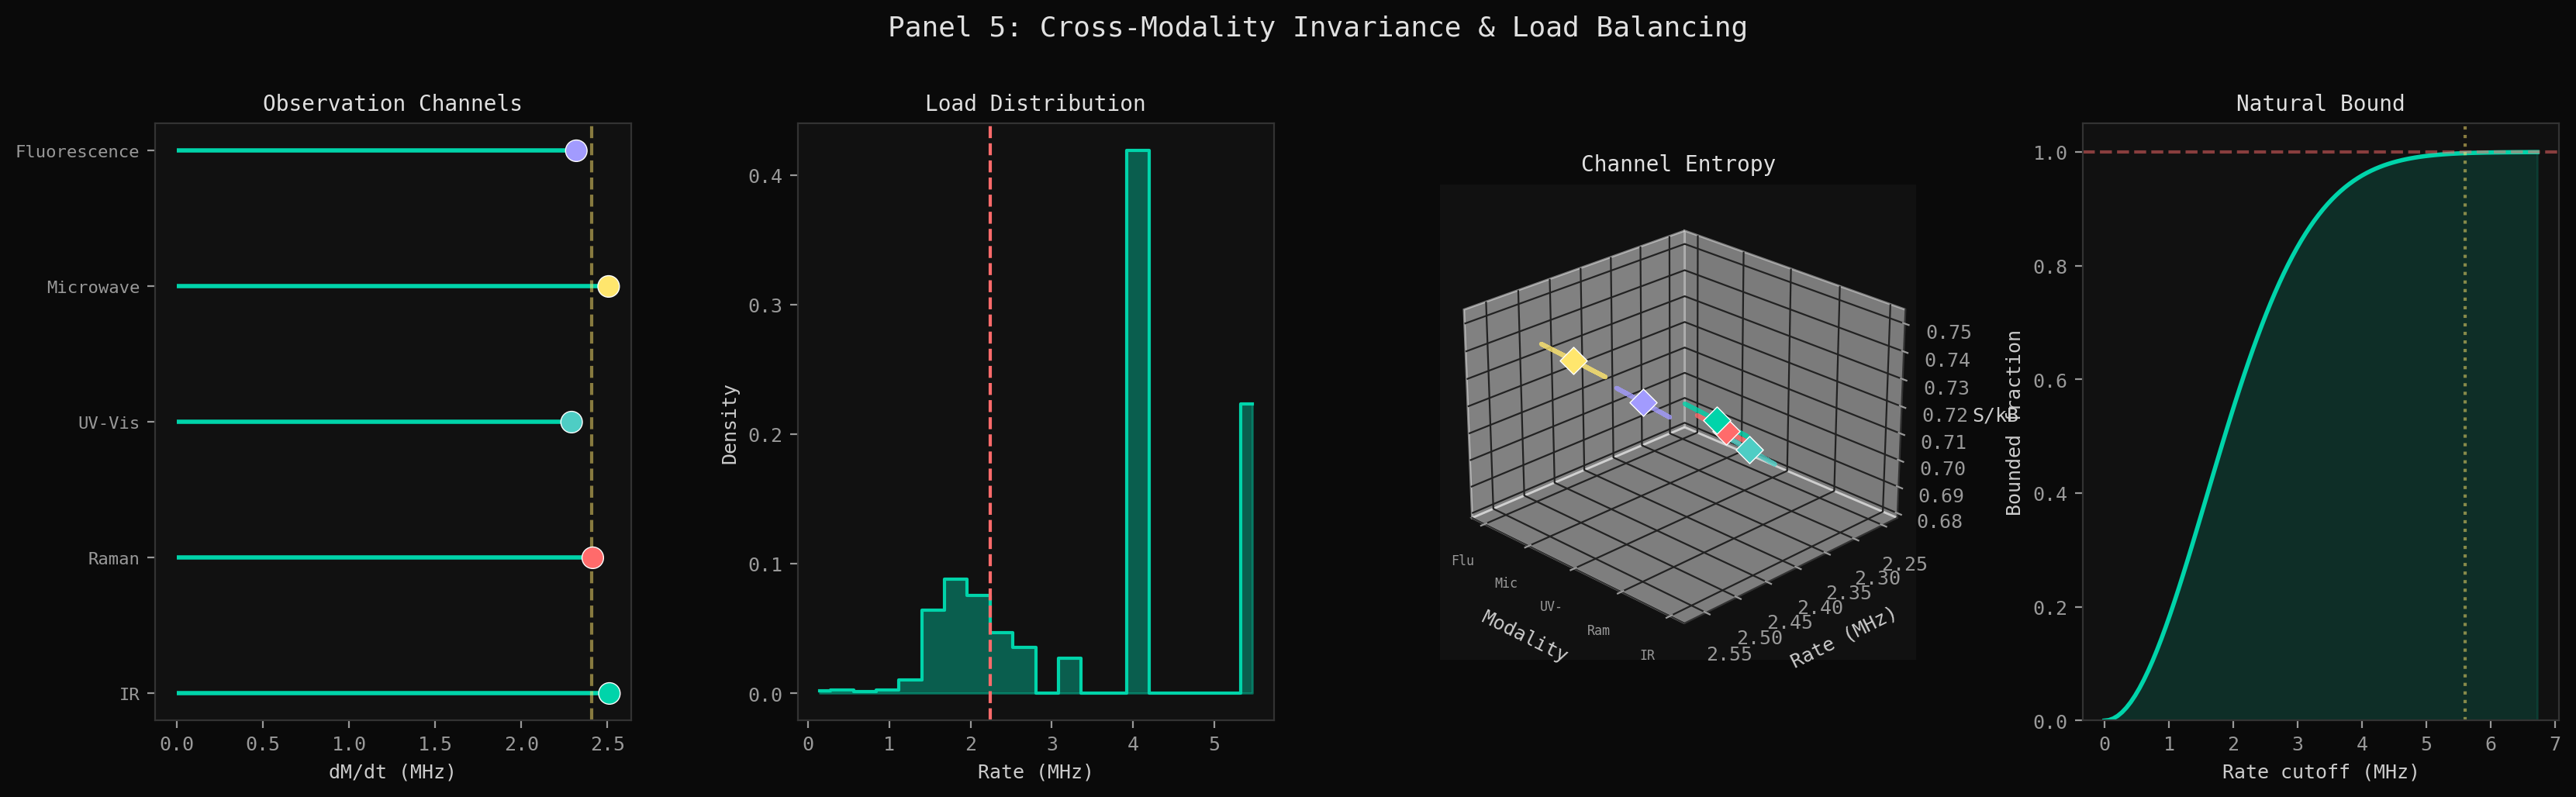
\includegraphics[width=\textwidth]{figures/panel5_modality_distribution.png}
    \caption{\textbf{Cross-Modality Invariance and Computational Load Balancing.}
    (\textbf{A})~Categorical transition rates $dM/dt$ measured through five independent spectroscopic observation channels: IR ($\Delta\ell = \pm 1$), Raman ($\Delta\ell = 0, \pm 2$), UV-Vis ($\Delta n$), Microwave ($\Delta m$), and Fluorescence ($\Delta s$). Lollipop markers (coloured by modality) cluster around the mean rate (dashed yellow line) with cross-modality $\mathrm{CV} = 4.25\%$, confirming that the computational identity is observer-invariant.
    (\textbf{B})~Rate distribution (histogram) for the $N = 100$ virtual gas ensemble, showing the Maxwell--Boltzmann load profile. The dashed red line marks the mean rate. The distribution exhibits the characteristic asymmetric shape with a bounded upper tail---computational load is naturally self-balancing.
    (\textbf{C})~Three-dimensional channel entropy: entropy per modality $S/k_B$ plotted over the modality--rate plane. Each coloured trace shows rate fluctuations (horizontal oscillation) and corresponding entropy (vertical position) for one observation channel. Diamond markers indicate the mean entropy per channel. The near-equal entropy levels across modalities confirm that observation channel choice does not bias the computational measurement.
    (\textbf{D})~Bounded fraction as a function of rate cutoff (CDF of the Rayleigh distribution). The fraction rises smoothly to $1.0$ (dashed red) at a finite cutoff, confirming the natural velocity bound. The dotted yellow vertical line marks the $2.5\bar{R}$ practical cutoff. No rates exist beyond the bound---the infinite velocity tail of classical kinetic theory is eliminated by the finite partition structure.}
    \label{fig:modality_distribution}
\end{figure*}
